\title{Midterm 2 for Algebra-Based Physics: Electricity and Magnetism}
\author{Dr. Jordan Hanson - Whittier College Dept. of Physics and Astronomy}
\date{\today}
\documentclass[10pt]{article}
\usepackage[margin=1.5cm]{geometry}
\usepackage{outlines}
\usepackage{graphicx}
\begin{document}
\maketitle

\section{Equations and constants}

\begin{enumerate}
\item Kirchhoff's Rules: 1) $I_{in} + I_{out} = 0$ (Junction Rule) 2) $\sum_{loop} V_i = 0$ (Loop Rule)
\item Ohm's Law: $V = IR$
\item Power from current: $P=IV$
\item Voltage in an RC across the capacitor: $V(t) = \epsilon\left(1 - \exp\left(-t/\tau\right)\right)$, where $\epsilon$ is the battery voltage and $\tau = RC$.
\item Lorentz Force: $\vec{F} = q \vec{v} \times \vec{B} = I \vec{L} \times \vec{B}$.
\item Centripetal force: $F_C = mv^2/r$.
\item Magnetic torque: $\vec{\tau}_B = \vec{\mu} \times \vec{B}$
\item Magnitude of torque: $|\vec{\tau}_B| = \mu B \sin\theta$
\item Magnetic dipole moment: $\vec{\mu} = I \vec{A}$ (the current times the area vector)
\item Magnetic field at the center of a current-carrying loop: $\vec{B} = (\mu_0 I)/(2 R)\hat{z}$, if the current is in the x-y plane.
\item Ampere's Law: $\int \vec{B} \cdot d\vec{s} = \mu_0 I_{enc}$ which is $B S = \mu_0 I_{enc}$ for simple cases where B is constant around the path, and parallel to $d\vec{s}$.
\item Magnetic permeability: $\mu_0 = 4\pi \times 10^{-7}$ T m A$^{-1}$.
\item Mass of electron: $m_e = 9.1 \times 10^{-31}$ kg.
\end{enumerate}

\clearpage

\section{Exercises}

\begin{enumerate}
\item \textbf{Chapter 10: DC Circuits and Kirchhoff's Rules}
\begin{enumerate}
\item 
\begin{figure}[ht]
\centering
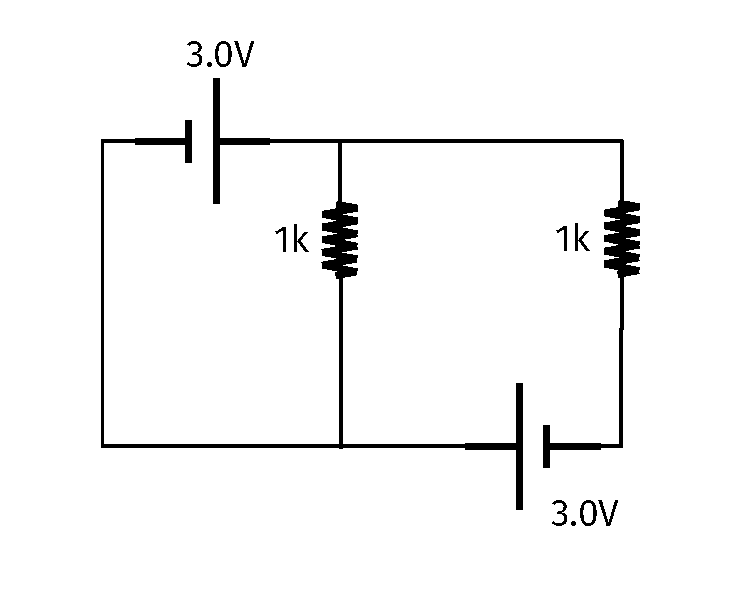
\includegraphics[width=0.5\textwidth]{iV.pdf}
\caption{\label{fig:circuit1} A circuit with three resistors powered by two voltages.}
\end{figure}
What are the currents flowing through each resistor in Fig. \ref{fig:circuit1}? \textit{Hint: first define the current in each segment of the circuit.  Then apply the junction rule once and the loop rule twice.}\\ \vspace{10cm}
\item An RC circuit has a time constant $\tau = 1$ ms.  If the resistance is $R = 1$ k$\Omega$, what is the value of the capacitor? \\ \vspace{3cm}
\end{enumerate}
\item \textbf{Chapter 11: Magnetic forces and fields}
\begin{enumerate}
\item A cosmic-ray electron moves at $2 \times 10^7$ m/s at a 90 degree angle to the Earth’s magnetic field at an altitude where the field strength is $2.0 \times 10^{-4}$ T. How long does it take to go in a circle? \\ \vspace{3 cm}
\item Calculate the maximum torque that can be achieved with a 200-turn square loop 20.0 cm on a side carrying a 30.0 A current, in a magnetic field of 1.0 T. \\ \vspace{2cm}
\end{enumerate}
\item \textbf{Chapter 12: Sources of Magnetic Fields}
\begin{enumerate}
\item What is the magnetic field produced at the center of a coil of wire with radius 5 cm, that has 100 turns, carrying a current of 0.5 A? \\ \vspace{2 cm}
\item What is the total magnetic dipole moment of a coil of wire that has 100 turns, carries 0.1 A of current, and has a radius of 1.0 cm? \\ \vspace{2cm}
\item
\begin{figure}[hb]
\centering
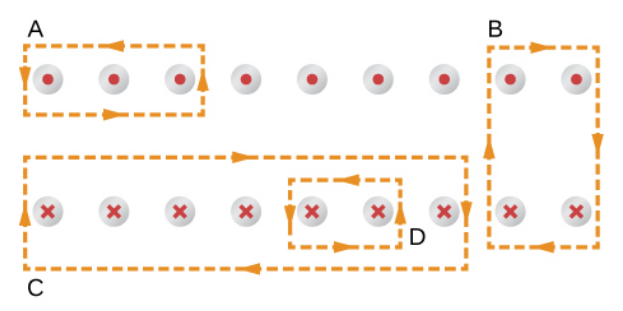
\includegraphics[width=0.3\textwidth]{circuit2.png}
\caption{\label{fig:circuit2} Several paths above correspond to line-integrals around a solenoid.}
\end{figure}
The coil whose lengthwise cross section is shown in Fig. \ref{fig:circuit2} carries a current I and has N evenly spaced turns distributed along the length L. Evaluate $\oint \vec{B} \cdot d\vec{l}$ for the paths indicated.
\end{enumerate}
\end{enumerate}
\end{document}